\documentclass[12pt]{article}

\usepackage{url}
\usepackage{fullpage}
\usepackage{graphicx}
\usepackage{amsmath,amssymb}

\newcommand{\eps}{\varepsilon}
\newcommand{\R}{\mathbb{R}}
\newcommand{\inprod}[1]{\langle #1 \rangle}

\DeclareMathOperator*{\E}{\mathbb{E}}
\let\Pr\relax
\DeclareMathOperator*{\Pr}{\mathbb{P}}

\begin{document}

\thispagestyle{empty}

\begin{center}
{\Large \textsc{CS 226 / 6.889 Sketching Algorithms for Big Data} --- Fall 2017}

\bigskip

{\Large \textsc{Problem Set 1}}

\smallskip

Due: 11:59pm, Monday, October 2nd

Submit to: \url{sketchingbigdata-f17-assignments@seas.harvard.edu}

\bigskip

{\footnotesize See homework policy at \url{http://www.sketchingbigdata.org/fall17/syllabus/}}
\end{center}

\paragraph{Preamble:} As you probably noticed, this pset is long. It does not mean it is difficult. The length is mostly due to the fact that the problems introduce additional material and concepts that (we believe) are interesting and shed new light on the material seen in the lecture.  If you have any questions about the new material, please contact the TA or the professors. 

\paragraph{Problem 1: More on incoherent matrices.} Recall from the JL lower bound lecture that an $\eps$-incoherent matrix $\Pi\in\R^{m\times n}$ is such that each column $\Pi^i$ of $\Pi$ has unit $\ell_2$ norm (i.e.\ $\sum_{j=1}^m (\Pi^i)_j^2 = 1$), and the dot products $\inprod{\Pi^i, \Pi^j}$ are all at most $\eps$ in magnitude for $i\neq j$. 

\begin{itemize}
\item[(a)] (3 points) In Lecture 5 we stated that an $n\times n$ real symmetric ``$\eps$-approximate identity'' matrix $A$ (with $1$'s on the diagonal and $\pm\eps$ on the off-diagonal entries) has rank $\Omega(n)$ if $\eps < 1/\sqrt{n}$. Let $A^{\oplus k}\in\R^{n\times n}$ be defined such that $(A^{\oplus k})_{i,j} = (A_{i,j})^k$. Show that if $r:=\mathop{rank}(A)$, then $\mathop{rank}(A^{\oplus k}) \le \binom{r+k}k$. Deduce a dimension lower bound of $m = \Omega(\min\{n,\eps^{-2}\log n / \log(1/\eps)\})$ for $(1+\eps)$-dimensionality reduction on the simplex.
\item[(b)] (2 points) In class we observed that any $(1+\eps)$-distortion embedding of the simplex $X = \{0,e_1,\ldots,e_n\} \subset\R^n$ gives an $O(\eps)$-incoherent matrix. Conversely, any $\eps$-incoherent matrix $\Pi$ gives a $(1+\eps)$-distortion embedding of the simplex (map $0$ to $0$, and $e_i$ to $\Pi^i$). Noga Alon's lower bound showed that any $\eps$-incoherent matrix with $m$ rows needs $m \gtrsim \min\{n, \eps^{-2}\lg n / \lg(1/\eps)\}$. This construction gives a hard point set of size $n+1$ in dimension $n$ for any $n$ (or said differently, a hard point set of size $n$ in dimension $d = n-1$). Show how to use Alon's approach to show that for any $d < n \le 2^{O(\eps^2 d)}$, there is a hard point set such that any $(1+\eps)$-distortion embedding into $m$-dimensional Euclidean space requires $m \gtrsim \min\{n, \eps^{-2}\lg n / \lg(1/\eps)\}$.
\end{itemize}

One way to construct an incoherent matrix is from a {\em code}. In particular, if $\mathcal{C} = \{C_1,\ldots,C_N\}$ is a collection of $N$ vectors each in $[q]^t$ for some positive integers $q,t$ (where $[q]$ denotes $\{1,\ldots,q\}$), then define $\alpha\in(0,1)$ as the maximum fraction of the $t$ coordinates for which any distinct $C_i,C_j$ agree. Given such a code, one can construct an $\eps$-incoherent matrix with $m = qt$, $n = N$, and $\eps=\alpha$ as in Figure~\ref{fig:codes}.  Note the dot product between two different codewords is exactly the fraction of coordinates on which they agree.

\begin{figure}[!h]
\begin{center}
\scalebox{0.8}{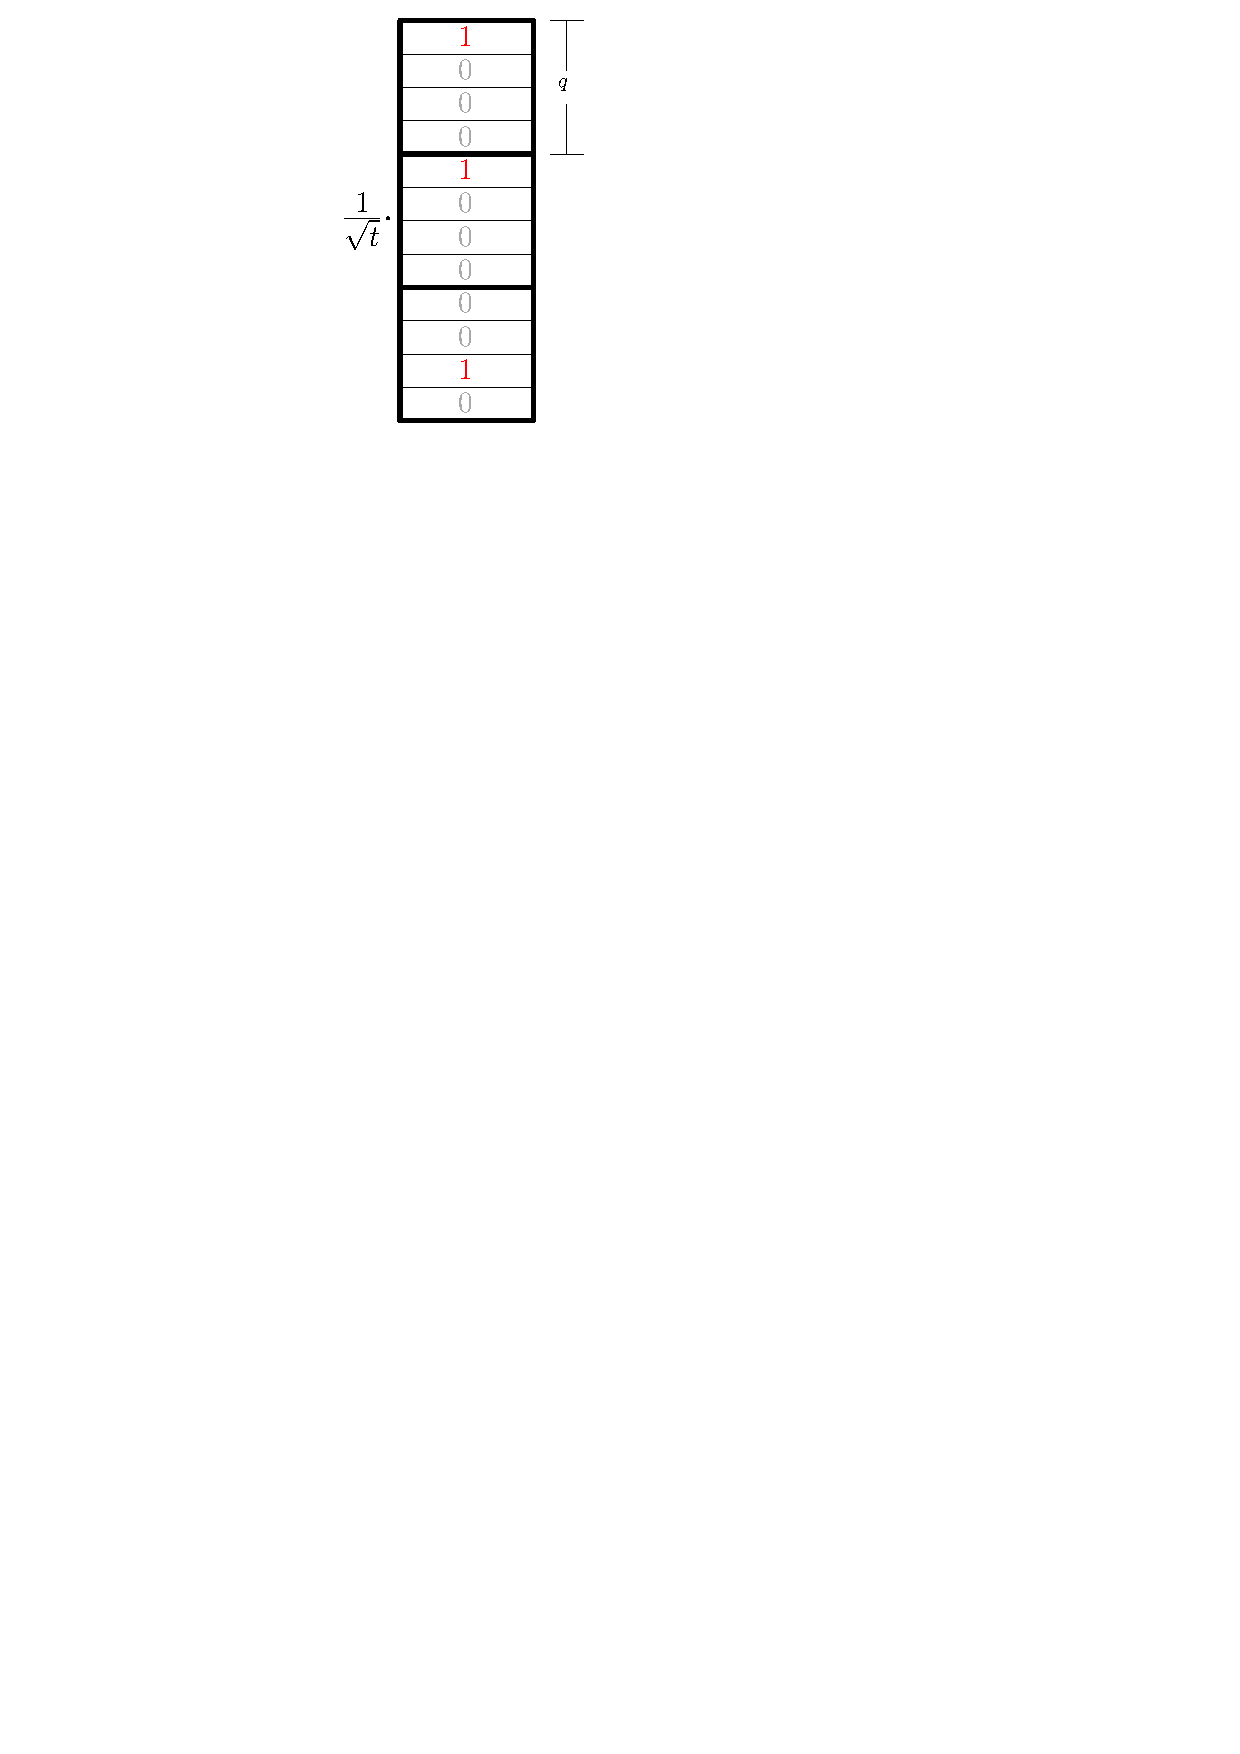
\includegraphics{code_vector}}
\caption{Each codeword gives one column of the incoherent matrix. Here $q = 4, t = 3$ and the codeword is $C_i = (1,1,3)$. The vector is $m = qt$ dimensional with the coordinates broken up into $t$ blocks each of size $q$. A $1$ is placed in the $j$th position in the location specified by $(C_i)_j$. The entire vector is normalized by $1/\sqrt{t}$ to have unit norm.}\label{fig:codes}
\end{center}
\end{figure}

We would like to show how to construct a code that gives small $m=qt$.

\begin{itemize}
\item[(c)] (3 points) Show that for any $N$ and $0<\alpha<1/2$, such codes exist with $q = O(\alpha^{-1}), t = O(\alpha^{-1}\log N)$ by picking random $C_i$ (hint: use the Chernoff bound). Note this gives an incoherent matrix with $N$ columns and $m = qt = O(\eps^{-2}\log N)$ rows, matching JL.
\end{itemize}

It turns out one can do better when $\eps$ is sufficiently small. Consider the finite field $\mathbb{F}_q$ and consider all polynomials $p_1,\ldots,p_N\in \mathbb{F}_q[x]$ of degree at most $d$ where $N = q^{d+1}$. Define the {\em Reed-Solomon code} $C_1,\ldots,C_N$ as follows: $t = q$ where the $j$th entry of $C_i$ is the evaluation of $p_i$ on the $j$th element of $\mathbb{F}_q$ (so $C_i$ is the evaluation table of $p_i$).

\begin{itemize}
\item[(d)] (6 points) Recall we need $N \ge n$ to ensure there are enough $C_i$'s to form our matrix $\Pi$. Show how to choose $d,q$ so $N \ge n$ and $\alpha \le \eps$, and show what this gives (in big-Oh notation) for $m = qt$ being the number of rows over the incoherent matrix $\Pi$ we obtain.
\item[(e)] (4 points) How small does $\eps$ need to be as a function of $n$ for the codes from part (d) to give smaller $m$ than the random codes from part (c)? If the turning point is $\eps_T$, you should provide an answer $\eps'_T$ such that $\log(1/\eps'_T) = \Theta(\log(1/\eps_T))$.
\item[(f)] (5 points) Suppose one has an $\eps$-incoherent matrix $\Pi$. Show how $\ell_1$-point queries to $x$ being updated in the turnstile streaming model can be answered solely given $y = \Pi x$. (Note then that part (d) implies a {\em deterministic} $\ell_1$-point query algorithm with low space in turnstile streams.) \textbf{Hint:} it may  help to remember that $\Pi x = \sum_i x_i \Pi^i$.
\end{itemize}

\noindent \textbf{OPEN PROBLEM:} As mentioned above, an incoherent matrix with $m = O(\eps^{-2}\log n)$ exists. The solution to this problem provides another, incomparable bound. The lower bound is $m = \Omega(\min\{n, \eps^{-2}(\log n)/\log(1/\eps))\}$ \cite[Section 9]{Alon03}. Can the gap between upper and lower bounds be closed? It is conceivable a better upper bound could be achieved by discovering a better code construction.

\paragraph{Problem 2: Counting distinct elements with deletions.}  In Lecture 2 we showed how to estimate the number of distinct elements in a stream in $\mathop{poly}(\eps^{-1}\lg n)$ bits of space with $2/3$ success probability, where all integers in the stream are in $[n]$. As mentioned in Lecture 3, this problem can be re-cast in the following way: there is a vector $x\in\R^n$ that starts as $0$, and each integer $i$ in the stream causes the change $x_i \leftarrow x_i + 1$. We would then like to estimate $\|x\|_0 := |\{i : x_i\neq 0\}|$. What if the updates in the stream are of the form $(i,\Delta)$ for $\Delta\in\{-1,1\}$, and now such an update causes the change $x_i\leftarrow x_i + \Delta$?

\begin{itemize}
\item[(a)] (2 points) What about our non-idealized algorithm from Lecture 2 breaks down now that negative updates are also allowed?
\item[(b)] (8 points) Show how to alter the non-idealized algorithm to obtain space $\mathop{poly}(\eps^{-1}\lg (nm))$ for this modified problem, where $m$ is the length of the stream. \textbf{Hint:} consider using techniques from Lecture 7 to fix the issue in part (a).
\end{itemize}

\paragraph{Problem 3: Reducing randomness via Nisan's Generator.}

In Lecture 4 we have seen a collection of algorithms for estimating the $\ell_p$ norm of the $n$-dimensional vector $x$ induced by the stream, for $p \in (0,2]$. The idea was to calculate a ``linear sketch'' $\Pi x=[Z_1 \ldots Z_k]$, where $R$ was an $k \times n$ random matrix, with i.i.d. entries $r_{ij}$ selected from a $p$-stable distribution. After calculating $\Pi x$,  the algorithm outputs  

\[ \text{median}[ |Z_1|, \cdots , |Z_k| ]/C(p) \]
as an estimator of $\|x\|_p$, where $C(p)$ denotes some scaling factor that depends only on $p$. To make life simple, in this problem we will focus on the decision version of the algorithm, which checks whether

\begin{eqnarray}
\text{median}[ |Z_1|, \cdots , |Z_k| ]/C(p) &  \ge &  T 
\label{a:test}
\end{eqnarray}
for some threshold $T$.  
For concreteness, in what follows we focus on $p=2$, in which case the entries of $\Pi$ can be selected from Gaussian distribution $\mathcal N(0,1)$. We also assume that the entries of $x$ always remain integers from $\{-M \ldots M\}$ for some $M=n^{O(1)}$, i.e., they have values polynomial in the dimension $n$.  

The analysis in the lecture skipped over the following two issues:
\begin{itemize}
\item Discretization: given that the algorithm space is measured in bits, we need to make sure that each $r_{ij}$ has  bounded precision. Dealing with this issue is  straightforward, as we can modify the random variables so that their values fall into an interval $[-C \sqrt{\log n} \ldots C \sqrt{\log n} ]$, and are multiples of of $1/n^C$, for some  $C=O(1)$. The analysis of the modified algorithm remains essentially unchanged, modulo minor increase in the approximation error and failure probability. In what follows we assume that $r_{ij}$ are already generated in this way, and therefore need only $b=O(\log n)$ bits of representation. 
\item Pseudo-randomness: even if $r_{ij}'s$ are discrete, we cannot afford to store all of them in memory, as this would require $knb$ bits of storage. Instead, it was mentioned that they can be generated ``on the fly'' using a pseudorandom generator, i.e., there is an efficiently computable mapping $G:\{0,1\}^L \to \{ \{0,1\}^b \}^{nk}$ such that we can set $r_{ij}=G(v)_{ij}$, where $v$ is a ``random seed'' selected from $\{0,1\}^L$ uniformly at random.  Formalizing and optimizing this step is the focus of this problem. 
\end{itemize}


We will use the pseudo-random generator for bounded space due to Nisan \cite{Nisan92}. Consider a class of {\em $(S,b)$-automata} $Q$, that have $2^S$ states and read sequences of symbols from $\{0,1\}^b$, i.e., operate over an alphabet of size $2^b$. 
Such automata are defined by:
\begin{itemize} 
\item  a transition function $Q(s,a)$, which descibe the state the automaton moves to from state $s$ after reading $a$,
\item  an initial state $start$, and 
\item a set of accepting states $Acc$.
\end{itemize}
 Such automata can model any deterministic computation device  that processes a sequence $u$ of symbols  from $\{0,1\}^b$ in space $S$. We use $Q(u)$ to denote the state reached by the automaton  after reading $u$, starting from $start$.

Nisan's generator $G$ has the following wonderful properties. Suppose that the automaton is applied to  sequences of length $R$. Then:
\begin{itemize}
\item The seed length $L$  of $G$ is equal to $O(S \log R)$, assuming $b=O(S)$.
\item It {\em $\epsilon$-fools} any $(S,b)$-automaton $Q$  , i.e., 
\[ 
|\Pr_{u \in (\{0,1\}^b)^R} [ Q(u) \in Acc] - \Pr_{v \in \{0,1\}^L } [ Q(G(v)) \in Acc] | \le \epsilon 
\]
for $\epsilon=2^{-\Omega(S)}$.
\end{itemize}
Note that in the above definition, the input to $Q$ consists of (pseudo)-random bits, which are ``tested'' by $Q$. Nisan's generator is designed to $\epsilon$-fool all such tests, despite generating randomness from a relatively small truly random seed. 

To use Nisan's generator in our streaming algorithm, we need to model the algorithm as a finite automaton reading the random entries of the matrix $\Pi$ and producing some decision in the end. Then we use the properties of the generator to argue that replacing truly random $\Pi$ by a pseudorandomly generated version does not (significantly) alter the behavior of the algorithm. 

 The computation specified in Equation~\eqref{a:test} can be performed by an automaton $Q$ that reads the entries  $r_{1,1}, \ldots , r_{1,n}, r_{2,1}, \ldots , r_{2,n}, \ldots r_{k,n}$ of $\Pi$ (i.e., in the row-wise order), computes the vector $[ Z_1, \cdots , Z_k ]$, evaluates the median and accepts if the result is at least  $T$. (Note that $Q$ is {\em parameterized} by the vector $x$, i.e., $x$ is {\em not} an input to $Q$!).

Finally, we are ready to state the problems:

\begin{itemize}
\item[(a)] (3 points) Observe that $Q$ can be implemented so that $S=O( k \log n)$. Calculate the length of the seed $L$ required to $2^{-\Omega(S)}$-fool such automata $Q$.
\item [(b)] (12 points) Show a better implementation of $Q$ that requires only $S=O( \log k + \log n)$. Calculate the length of the seed $L$ required to $2^{-\Omega(S)}$-fool such automata $Q$.
\end{itemize}


\paragraph{Problem 4:} (1 point) How much time did you spend on this problem set? If you can remember the breakdown, please report this per problem. (sum of time spent solving problem and typing up your solution)

\bibliographystyle{alpha}

\begin{thebibliography}{42}

\bibitem{Alon03}
Noga Alon.
\newblock Problems and results in extremal combinatorics--I
\newblock {\em Discrete Mathematics}, 273(1-3): 31--53, 2003.

\bibitem{Nisan92}
Noam~Nisan.
\newblock Pseudorandom Generators for Space-Bounded Computation.
\newblock {\em Combinatorica}, 12(4):449-461, 1992.

\end{thebibliography}

\end{document}


\paragraph{Problem 3: The Johnson-Lindenstrauss lemma with $\pm 1$ random variables.} In Lecture 4, we showed that if $\Pi\in\R^{m\times n}$ has i.i.d.\ $\mathcal N(0, 1/m)$ entries, then we obtain the distributional JL lemma guarantee (here $\mathcal N(\mu, \sigma^2)$ is the normal distribution with mean $\mu$ and variance $\sigma^2$). We would like to show that it even suffices for $\Pi$ to have entries which are independent and uniform in $\{-1/\sqrt m, 1/\sqrt m\}$.

Define $\psi_Z(\lambda) = \ln \E e^{\lambda Z}$. A random variable $Z$ is {\em $\sigma$-subgaussian} if $\psi_Z(\lambda) \le \lambda^2\sigma^2/2$ for all $\lambda\in \R$. It is {\em $(\sigma,B)$-subgamma} if $\psi_{|Z|}(\lambda)  \le \lambda^2\sigma^2/2$ for all $|\lambda|< 1/B$. Define $\|Z\|_p := (\E |Z|^p)^{1/p}$. You may use without proof that this is a norm for $p\ge 1$ (Minkowski's inequality).

\begin{itemize}
\item[(a)] (3 points) Show that the following two properties are equivalent to being $\sigma$-subgaussian, up to potentially changing $\sigma$ by a constant factor.
\begin{itemize}
\item[$\bullet$] $\Pr(|Z| > t) < 2e^{-t^2/(2\sigma^2)}$ for all $t>0$
\item[$\bullet$] $\|Z\|_p \le \sigma\sqrt p$ for all $p\ge 1$
\end{itemize}
\item[(b)] (3 points) A random variable is {\em $\sigma$-subexponential} if it is $(\sigma^2, \sigma)$-subgamma. Show that the following two properties are equivalent to being $\sigma$-subexponential, up to potentially changing $\sigma$ by constant factors.
\begin{itemize}
\item[$\bullet$] $\Pr(|Z| > t) < 2 e^{-t/(2\sigma)}$ for all $t>0$
\item[$\bullet$] $\|Z\|_p \le \sigma p$ for all $p\ge 1$
\end{itemize}
\item[(c)] (2 points) Show that if $Z$ is $\sigma$-subgaussian, then $Z^2$ is $C\sigma$-subexponential for some universal constant $C$. \textbf{Hint:} you may want to use that if $X$ is $\sigma$-subexponential, then $X-\E X$ is $C\sigma$-subexponential. This follows by 3(c) and using the fact that 
\begin{align*}
\|X - \E X\|_p &= \|X - \E Y\|_p\text{ (}Y\text{ is an independent copy of }X\text{)}\\
{}& \le \|X - Y\|_p\text{ (Jensen's inequality)}\\
{}&\le \|X\|_p +\|Y\|_p \text{ (triangle inequality)}\\
{}&= 2\|X\|_p
\end{align*}
\item[(d)] (4 points) Show that if $X_1,\ldots,X_n$ are independent with $X_i$ being $(\sigma_i, B_i)$-subgamma, then $\sum_{i=1}^n X_i$ is $(\sqrt{\sum_i \sigma_i^2}, \min_i B_i)$-subgamma.
\item[(e)] (3 points) Show that if $Z$ is $(\sigma, B)$-subgamma, then $\Pr(|Z - \E Z| > t) < 2 \max\{e^{-Ct^2/\sigma^2}, e^{-t/2B}\}$ for all $t>0$, for some universal constant $C$.
\item[(f)] (5 points) Conclude that the distributional JL lemma holds even if the entries of $\Pi\in\R^{m\times n}$ are i.i.d.\ in $\{-1/\sqrt{m}, 1/\sqrt m\}$, where $m = O(\eps^{-2}\log(1/\delta))$.
\end{itemize}

